 % !Mode:: "TeX:UTF-8"
%% 请使用 XeLaTeX 编译本文.
%% 模板修改时间:2017-04-20, powered by daiao
%\documentclass[UTF8]{WHUMaster-chapter-center}   
\documentclass[]{WHUMaster-chapter-center} % 选项 forprint: 交付打印时, 建议加上此选项, 以消除彩色链接文字, 避免彩色字迹打印偏淡.
                                              % 选项 forlib: 提交给图书馆的电子版, 需要加上选项 forlib, 以消除空白页和彩色链接.
                                              % 选项 smd: Specialist Master's Degree, 产生专业硕士学位论文封面、页眉.
%%%=== 参考文献=== %%%
%\usepackage[T1]{fontenc}
\usepackage{textcomp}
\usepackage{makecell}
\usepackage{booktabs}  
\usepackage{threeparttable} 
\usepackage{multirow} 
%\usepackage[top=2cm, bottom=2cm, left=2cm, right=2cm]{geometry}  
\usepackage{algorithm}  
\usepackage{algorithmicx}  
\usepackage{algpseudocode}  
\usepackage{amsmath}  
\usepackage{float}
\usepackage{makecell}
%\usepackage{subfigure}
\usepackage[T1]{fontenc} %设置times new roman
\usepackage{mathptmx}  %设置times new roman
\usepackage{hyperref}
\usepackage{url}
\usepackage{epstopdf}
\usepackage{bm}
\hypersetup{
    colorlinks=true,
    linkcolor=black,
    filecolor=black,      
    urlcolor=black,
    citecolor=black,
}
\usepackage{booktabs} % 用于三线表
\captionsetup{font={normalsize}}
\bibliographystyle{gbt7714-2005-wuda-20170408}        % 参考文献样式,  plain,unsrt,alpha,abbrv 等等

%%%  He begin %%%%%%%
\usepackage{enumerate}
\usepackage{enumitem} 
\usepackage{caption}
\usepackage[justification=centering]{subcaption}
\usepackage{pifont}
\newcommand{\True}{\ding{52}}
\newcommand{\False}{\ding{56}}
\usepackage[super]{nth}
\captionsetup{labelsep=space}  %去除冒号
%%%%% He end    %%%%%%%%%%%%%%%
%\begin{figure}[!htbp]
%其中htbp是可选的,它们分别代表
%!-忽略“美学”标准
%h-here
%t-top
%b-bottom
%p-page-of-its-own
%%%%%%%%%%%%%%%%%%%%%%%%%%%%%%%%%%%%%%%%%%%%%%%%%%%%
\begin{document}
%%%%%%%-------------------------------------------------
\fenleihao{TN911~~~}  % 分类号:《中国图书资料分类法》的类号. 必填. 要根据自己的学科方向填写!!
\miji{}                % 密级
\UDC{}               %《国际十进制分类法UDC》的类号. 选填.
\bianhao{10486~~~}  % 学校编号, 10486是武汉大学的编号. 不用改动.

\title{中文题目}
\Etitle{English Title} % 英文题目
\author{小何}
\StudentNumber{20182021xxxxx}   % 学号
\Eauthor{{\zihao{4}Achhhe}}            %作者英文名
\Csupervisor{小明\quad 教授}        %指导教师中文名、职称
\Esupervisor{Prof.~Ming Xiao}     %指导教师英文名、职称
\Cmajor{信息与通信工程}                          % 专业中文名[ SMD:专业类别(领域)]
\Emajor{Information and Communication Engineering }% 专业英文名[ SMD:专业类别(领域)]
\Cspeciality{图像复原}                     % 研究方向
\Especiality{Image Restoration}   % 研究方向
\Schoolname{School of Electronic Information} %学院英文名. 不确定的话, 请看一下自己学院的网页上是怎么写的. 别搞错了!
\date{二〇二一年五月}                    % 硕士类只写年月. 要注意和英文日期一致!!
\Edate{May, 2021}                   % 英文封面日期

%-----------------------------------------------------------------------------
\pdfbookmark[0]{封面}{title}         % 封面页加到 pdf 书签
\maketitle
%---------------------r1--------------------------------------------------------
% !Mode:: "TeX:UTF-8"

%%%%%%%%%%%%   modified by he 2021-4-13    %%%%%%%%%%%%%%%%%%
%%% 原latex模板封面与word版本不一样,此处添加word对应形式
%%%%%%%%%%%%%%%%%%%%%%%%%%%%%%%%%%%%%%%%%%%%%%%%%


%%% 此部分包含: (1) 英文封面 (无需改动) ; (2) 郑重声明 (无需改动).

%%%%%%%%%%%%%%%%%%%%%%%%%%%%%
%%% -------------  英文封面 (无需改动)-------------   %%%
%%%%%%%%%%%%%%%%%%%%%%%%%%%%%
\thispagestyle{empty}
\renewcommand{\baselinestretch}{1.5}  %下文的行距
\vspace*{0.5cm}

\begin{center}
  {\zihao{2} \textbf{MASTER'S DEGREE THESIS \\ OF WUHAN UNIVERSITY} \par}
\end{center}

\begin{center}{\zihao{5}  \par}\end{center}
\begin{center}{\zihao{5}  \par}\end{center}
\begin{center}{\zihao{5}  \par}\end{center}
\begin{center}{\zihao{5}  \par}\end{center}

\begin{center}{\zihao{2} \the\Etitle \par}\end{center}


\begin{center}{\zihao{5}  \par}\end{center}
\begin{center}{\zihao{5}  \par}\end{center}
\begin{center}{\zihao{5}  \par}\end{center}
\begin{center}{\zihao{5}  \par}\end{center}
\begin{center}{\zihao{5}  \par}\end{center}
\begin{center}{\zihao{5}  \par}\end{center}
\begin{center}{\zihao{5}  \par}\end{center}
\begin{center}{\zihao{5}  \par}\end{center}
\begin{center}{\zihao{5}  \par}\end{center}
\begin{center}{\zihao{5}  \par}\end{center}
\begin{center}{\zihao{5}  \par}\end{center}
\begin{center}{\zihao{5}  \par}\end{center}

\begin{center}{\zihao{4} By             \par}\end{center}
\begin{center}{\zihao{4} \the\Eauthor    \par}\end{center}
\begin{center}{\zihao{4} Supervised by    \par}\end{center}
\begin{center}{\zihao{4} \the\Esupervisor   \par}\end{center}

\begin{center}{\zihao{5}  \par}\end{center}
\begin{center}{\zihao{5}  \par}\end{center}
\begin{center}{\zihao{5}  \par}\end{center}
\begin{center}{\zihao{5}  \par}\end{center}

\begin{center}{\zihao{3} \the\Edate \par}\end{center}


%%%%%%%--判断是否需要空白页-----------------------------
  \iflib
  \else
  \newpage
  \thispagestyle{empty}
  \cleardoublepage
  \fi
%%%%%%%-------------------------------------------------
%%%--- 加入``郑重声明'' --- %%%%%%%%%%%%%%%%%
{\pagestyle{empty}
\newpage
\vspace*{20pt}
\begin{center}{\ziju{0.8}\zihao{-2}\heiti 论文原创性声明}\end{center}
\par\vspace*{30pt}
\renewcommand{\baselinestretch}{2}
{\zihao{4} \songti %


本人郑重声明: 所呈交的学位论文, 是本人在导师指导下, 独立进行研究工作所取得的研究成果.
除文中已经标明引用的内容外, 本论文不包含任何其他个人或集体已经发表或撰写过的研究成果.
对本文的研究做出贡献的个人和集体, 均已在文中以明确方式标明. 本声明的法律结果由本人承担.


\vskip2cm

\hspace*{4cm}学位论文作者(签名): \hspace{4cm} \hfill \\[1cm]
\hspace*{10cm}年 \hfill  月 \hfill 日\hspace{1cm}\hfill\par}

%%%%%%%--判断是否需要空白页-----------------------------
  \iflib
  \else
  \newpage
  \cleardoublepage
  \fi
%%%%%%%-------------------------------------------------
}
\renewcommand{\baselinestretch}{1.6}
\small\normalsize




    % 加入英文封面
\frontmatter
\pagenumbering{Roman}               % 正文之前的页码用大写罗马字母编号.

\cleardoublepage
\newpage  \pagestyle{fancy} \fancyfancy
%------------------------------------------------------------------------------
% !Mode:: "TeX:UTF-8"

%%% 说明: 此部分需要自己填写的内容:  (1) 中文摘要及关键词 (2) 英文摘要及关键词

%%%%%%%%%%%%%%%%%%%%%%%
%%% ------------ 中文摘要 ---------------%%%
%%%%%%%%%%%%%%%%%%%%%%%
\begin{cnabstract}

图像去雨旨在xxx。研究内容与贡献总结如下:


(1)xxx。


(2)xxx。

(3)xxx。

(4)xxx。 

\end{cnabstract}
%\vspace{1em}\par\vfill

\begin{center}{\songti\zihao{-4}  \par}\end{center}

%%%--------- 关键词 -------- %%%
\noindent\cnkeywords{\large { 单幅图像去雨,卷积稀疏编码,半监督学习} }
%%%%%%%%%%%%%%%%%%%%%%%


%%%%%%%%%%%%%%%%%%%%%%%
%%% ------------ 英文摘要 ---------------%%%
%%%%%%%%%%%%%%%%%%%%%%%

\begin{enabstract}
%This thesis is a study on the theory of \dots.
%英文摘要,注意用英文逗号

The major focus and contributions are as follows:


(1) xxxx.

(2) xxx.

(3) xxx. 


(4) xxx.
 


\end{enabstract}
%\vspace{1em}\par\vfill

\begin{center}{\songti\zihao{-4}  \par}\end{center}

%%%------ 英文关键词 ------- %%%
\noindent\enkeywords{{ single image deraining, convolutional sparse coding, semi-supervised learning}}


      % 加入中英文摘要.
%---把目录加入到书签---%%%%%%%%%%%%%%
\pdfbookmark[0]{目录}{toc}%%%%%%%%%%%%

\tableofcontents

%------------------------------------------------------------------------------
\mainmatter %% 以下是正文
\zihao{-4}
\baselineskip=20pt  % 正文行距为 20 磅
%\fontsize{12pt}
%%%%%%%%%%%%%%%%%%%%%r3%%%%%%%%%%%%%%%



\chapter{绪论}

无论使用texstudio还是vscode,建议
\begin{itemize}
	\item 分章节写,input进来,可以只编译当前章节,其他注释掉,节约编译时间,不然当工程比较大时,统一编译很慢
	\item 不同图片、表格也写在单独tex中,input进来
\end{itemize}

input进来的好处是看起来清爽,而且注释方便

\section{研究背景及意义}


\begin{table}[h]  
		\centering  
		\fontsize{10}{10}\selectfont  
		\caption{\rm 在Rain12\upcite{gmm}、Rain1200\upcite{didmdn}和Test1000\upcite{spanet}数据集上的定量结果(PSNR$\uparrow$与SSIM$\uparrow$)比较,$\uparrow$表示该评价指标数值越大算法性能越好,最佳与次佳结果分别用黑体和下划线标出。*表示本文所提方法。} 
		\label{tab:rain12-rain1200-test1000}
		\begin{threeparttable}  
			\begin{tabular}{c|cc|cc|cc}
				\toprule  
				\multirow{2}{*}{\makecell{Methods\\[-.15cm]}}& 
				\multicolumn{2}{c|}{Rain12}&\multicolumn{2}{c|}{Rain1200}&\multicolumn{2}{c}{Test1000}\cr  
				\cmidrule(lr){2-3} \cmidrule(lr){4-5}\cmidrule(lr){6-7}   
				&PSNR$\uparrow$ &SSIM$\uparrow$&PSNR$\uparrow$&SSIM$\uparrow$&PSNR$\uparrow$&SSIM$\uparrow$\cr  
				\midrule 
				 
				DSC\upcite{dsc}  &29.98&0.8654  &21.44&0.7896&32.33&0.9335\cr  
				GMM\upcite{gmm} &32.15&0.9145&22.75&0.8352&32.99&0.9475\cr 
				CNN~\upcite{cnn}   &33.33&0.9199&23.55&0.8352&31.31&0.9304\cr
				JORDER~\upcite{jorder}   & {36.15}&0.9548&25.71&0.8074&35.72&{0.9776}\cr
				DDN~\upcite{ddn}   & 29.84&0.9049& 30.08&0.8791&34.88&0.9727\cr 
				DID-MDN~\upcite{didmdn} &29.49&0.9031&29.65&0.9016&28.96&0.9457\cr
				%SEMI\upcite{semi} &- &-&26.05&0.8220&-&-\cr
				PreNet~\upcite{prenet} & \underline{36.66}&0.9610&30.56&0.8750&30.31&0.9538\cr
				SPANet~\upcite{spanet} &32.71 &0.9285&30.05&\bf 0.9342&38.53& \underline{0.9875}\cr
				\midrule
				CODE-Net* &{ 36.21}&\underline{ 0.9618}&{ \underline {33.31} }&0.9174&\underline{ 38.88}&0.9867\cr
				mCODE-Net*  &\bf { 36.79}&{ \bf {0.9639}}&{\bf {34.03}}&\underline{ 0.9281}&{\bf 39.85}&\bf 0.9879\cr  				
				\bottomrule  
			\end{tabular} 
		\end{threeparttable}  
\end{table}  

\begin{figure}[t] 
	\centering
	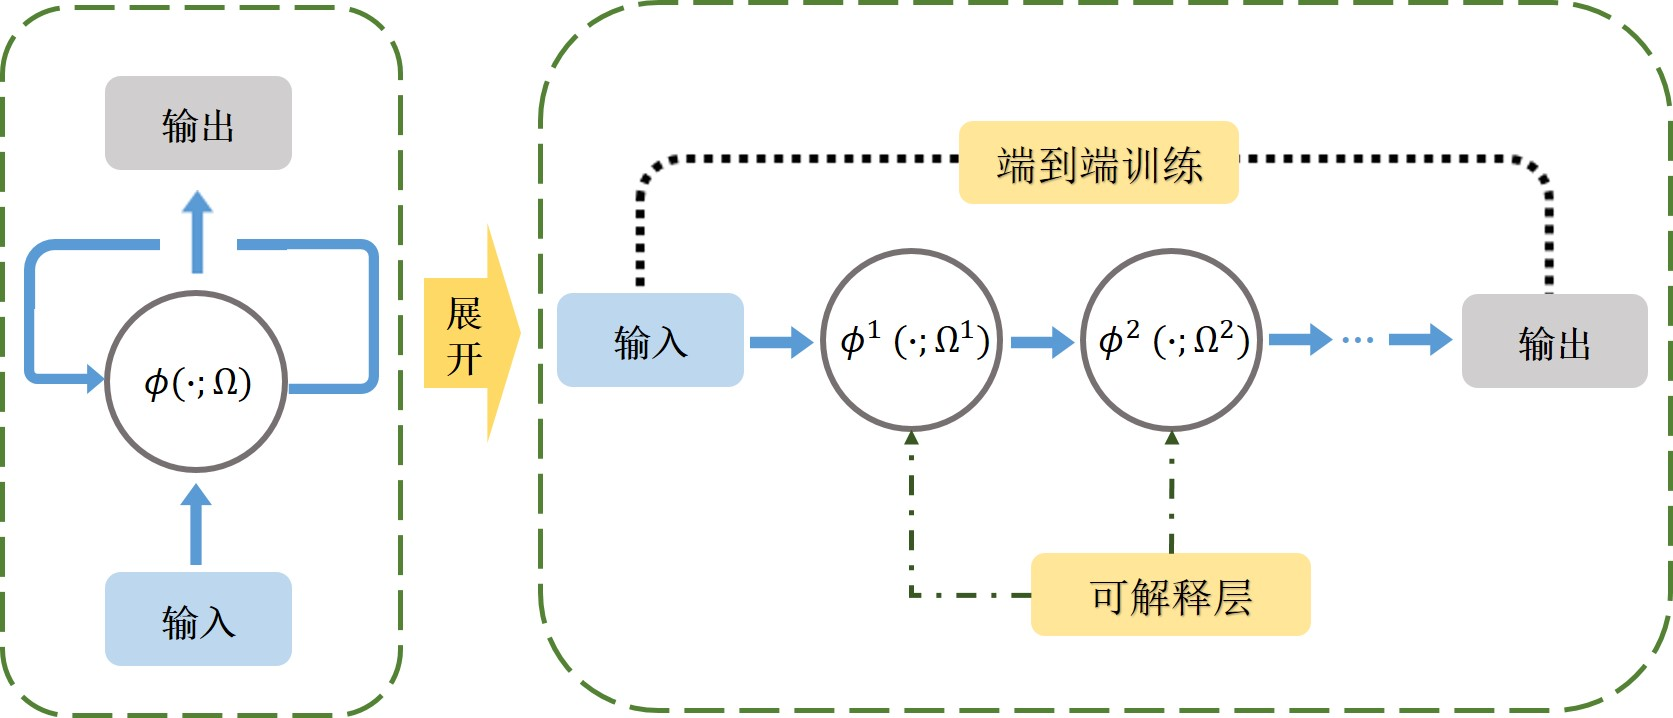
\includegraphics[width=0.99\linewidth]{figures/unroll.jpg}
	\caption{ \rm Deep Unfolding技术示意图。}
	\label{fig:unrolling}	
\end{figure} %

\chapter{图像去雨背景知识}
\section{引言}

 %

\chapter{基于连续雨强估计的自适应图像去雨算法}\label{chp3}
\section{引言}



 %

\chapter{基于循环一致性的半监督图像去雨算法}\label{chp4}
\section{引言}



 %

 \chapter{实验结果及分析}
 %

\chapter{总结与展望}
\section{论文总结}
%




%\section{论文电子版提交的格式问题}
%
%《武汉大学博、硕士研究生学位论文缴送办法》要求``电子版应采用~Word97 或~Word2000 格式(DOC)编辑 '\footnote{那已经是~2005 年的事情了.}.
%关于这个重要的问题, 我已致信武汉大学图书馆总馆信息服务中心袁晓川老师,
%得到的答复是: ``用~\LaTeX{} 软件排版的论文可直接提交~PDF 格式.''






%%%=== 参考文献 ========%%%
\cleardoublepage\phantomsection
\zihao{5}
\addcontentsline{toc}{chapter}{参考文献}

\bibliography{BIBbase/WHUMaster-bibtex}%%%加入路径中的参考文献.

\chapter*{攻读硕士期间科研成果}
\addcontentsline{toc}{chapter}{攻读硕士期间科研成果}

\section*{论文}
\begin{enumerate}[parsep=1.ex]
\renewcommand\labelenumi{[\theenumi]}  %% 给数字加上方括号
\item 
\textbf{XXX}, xxx, xxx, et al. Title[J]. Signal, Image and Video Processing (SIVP). Springer, 2021: x-x. (SCI, published)

\item 
\textbf{XXX}, xxx, xxx, et al. Title[J], IEEE Transactions on Multimedia (TMM). 2020. (SCI, published)

\item 
xxx*, \textbf{XXX}*, xxx, et al. Title[C]//European Conference on Computer Vision (ECCV). Springer, 2020: x-x. (CV Top, co-first author, published)

\item 
\textbf{XXX}, xxx and xxx. Title[C]//IEEE International Conference on Acoustics, Speech and Signal Processing (ICASSP). IEEE, 2020: x-x. (CCF-B, published)

\item 
xxx, \textbf{XXX}, xxx, et al. Title[C]//IEEE International Conference on Image Processing (ICIP). IEEE, 2020: x-x. (CCF-B, published)

\end{enumerate}

\section*{专利}
\begin{enumerate}[parsep=1.ex]
\renewcommand\labelenumi{[\theenumi]}  %% 给数字加上方括号
\item
xxx, \textbf{XXX}, xxx, xxx. Title. CN2019xxx.x[P]. 2019. (已授权, 导师一作)

\item
xxx, \textbf{XXX}, xxx, xxx. Title. CN2019xxx.x[P]. 2020.  (公开在审, 导师一作)


\item
xxx, xxx, \textbf{XXX}, xxx. Title. CN2020xxx.x[P]. 2020. (公开在审)

\item
xxx, xxx, \textbf{XXX}, xxx. Title. CN2019xxx.x[P]. 2019. (公开在审)

\end{enumerate}

\backmatter
% !Mode:: "TeX:UTF-8"

%%% 此部分内容:  (1) 致谢  (2) 武汉大学学位论文使用授权协议书(无需改动)

%%%%%%%%%%%%%%%%%%%%%%%
%%% --------------- 致谢 ------------- - %%%
%%%%%%%%%%%%%%%%%%%%%%%
\acknowledgement
\begin{normalsize}

三克油


\hfill Achhhe

\hfill 二零二一年四月

%\hfill 写于武汉大学珞珈山下
\end{normalsize}








%%%%%---武汉大学学位论文使用授权协议书---%%%%%%%%%%%%
%%%%%%%%%%%%%%%%%%%%%%%%%%%%%%%%%%%
%%%%%%%%%%%%%%%%%%%%%%%%%%%%%%%%%%%

%\cleardoublepage
%\newpage\vspace*{20pt}
%\begin{center}{\zihao{-2}\heiti 武汉大学学位论文使用授权协议书}\end{center}
%\par\vspace*{30pt}
%
%本学位论文作者愿意遵守武汉大学关于保存、使用学位论文的管理办法及规定,
%即:学校有权保存学位论文的印刷本和电子版, 并提供文献检索与阅览服务;
%学校可以采用影印、缩印、数字化或其它复制手段保存论文;
%在以教学与科研服务为目的前提下, 学校可以在校园网内公布部分及全部内容.
%\begin{enumerate}[1、]
%  \item  在本论文提交当年, 同意在校园网内以及中国高等教育文献保障系
%           统(CALIS)高校学位论文系统提供查询及前十六页浏览服务.
%  \item  在本论文提交~$\Box$~当年/~$\Box$~一年/~$\Box$~两年
%            /~$\Box$~三年/~$\Box$~五年以后, 同意在校园网内允许读者
%            在线浏览并下载全文, 学校可以为存在馆际合作关系的兄弟高校用
%            户提供文献传递服务和交换服务.(保密论文解密后遵守此规定)
%\end{enumerate}
%
%\vskip 15mm
%
%论文作者(签名):\raisebox{-1ex}{\underline{\makebox[5cm][c]{}}}
%\vskip2em
%				          				
%学\qquad\qquad\quad 号:\raisebox{-1ex}{\underline{\makebox[5cm][c]{}}}
%\vskip2em	
%					
%学\qquad\qquad\quad 院:\raisebox{-1ex}{\underline{\makebox[5cm][c]{}}}					
%
%\vskip  2cm
%\begin{flushright}
% 日期:\hskip2cm 年\hskip1.2cm 月\hskip1.2cm 日
%\end{flushright}

%%%%%%%%%%%%%%%%%%%%%%%%%%%%%%%%%%%%%%%
%%%%%%%--判断是否需要空白页-----------------------------
  %\iflib
  \ifsmd
  \else
  \newpage
  \cleardoublepage
  \fi
%%%%%%%-------------------------------------------------







 %%%致谢, 武汉大学学位论文使用授权协议书.
\cleardoublepage
\end{document}



